\documentclass{article}

\usepackage[spanish, activeacute]{babel} 
\usepackage[utf8]{inputenc}

\usepackage[]{minted}
\usepackage{natbib}
\usepackage{graphicx}
\usepackage{listings}

%Ruta absoluta en formato tipo Unix (Linux, OsX)
\graphicspath{ {./images/} }

\begin{document}

\title{Tutorial Raspberry Pi}
\author{David R Castañeda}
\date{\today}

\maketitle
sudo apt-get install texlive-lang-all

\section{Setear IP Fija}

De este tutorial para poner la IP fija en Raspbian tanto para el Ethernet, la red por cable, como para el Wi-Fi siguen funcionando, pero pueden dar lugar a configuraciones extrañas en que puede que veamos dos o más IP en nuestra red para una sola Raspberry Pi.

Todo esto se debe a que en las nuevas versiones de Raspbian las direcciones IP se gestionan con otro archivo de configuración, en concreto con dhcpcd.conf, además de un cambio mínimo en el fichero de interfaces. Configuramos primero uno de ellos, el nuevo con más cambios con el siguiente comando desde una Terminal:

sudo nano /etc/dhcpcd.conf
El fichero que se abre es este y la parte a añadir es justo la del final:

\begin{minted}[breaklines, frame=single, framesep=7pt]{bash}
# A sample configuration for dhcpcd.
# See dhcpcd.conf(5) for details.

# Allow users of this group to interact with dhcpcd via the control socket.
#controlgroup wheel

# Inform the DHCP server of our hostname for DDNS.
hostname

# Use the hardware address of the interface for the Client ID.
clientid
# or
# Use the same DUID + IAID as set in DHCPv6 for DHCPv4 ClientID as per RFC4361.
#duid

# Persist interface configuration when dhcpcd exits.
persistent

# Rapid commit support.
# Safe to enable by default because it requires the equivalent option set
# on the server to actually work.
option rapid_commit

# A list of options to request from the DHCP server.
option domain_name_servers, domain_name, domain_search, host_name
option classless_static_routes
# Most distributions have NTP support.
option ntp_servers
# Respect the network MTU.
# Some interface drivers reset when changing the MTU so disabled by default.
#option interface_mtu

# A ServerID is required by RFC2131.
require dhcp_server_identifier

# Generate Stable Private IPv6 Addresses instead of hardware based ones
slaac private

# A hook script is provided to lookup the hostname if not set by the DHCP
# server, but it should not be run by default.
nohook lookup-hostname

interface eth0
static ip_address=192.168.1.11
static routers=192.168.1.1
static domain_name_servers=8.8.8.8
static domain_search=8.8.4.4
\end{minted}

Os pongo un pantallazo marcando la parte añadida al final para tener la IP por cable fija:

Luego os tenéis que asegurar que en el archivo de interfaces está todo correcto para que la IP sea fija o estática o manual. Para ello usamos el siguiente comando desde una Terminal:

sudo nano /etc/network/interfaces
Y el fichero será algo así:

\begin{minted}[breaklines, frame=single, framesep=7pt]{bash}
# interfaces(5) file used by ifup(8) and ifdown(8)

# Please note that this file is written to be used with dhcpcd
# For static IP, consult /etc/dhcpcd.conf and 'man dhcpcd.conf'

# Include files from /etc/network/interfaces.d:
source-directory /etc/network/interfaces.d

auto lo
iface lo inet loopback

iface eth0 inet manual

allow-hotplug wlan0
iface wlan0 inet manual
    wpa-conf /etc/wpa_supplicant/wpa_supplicant.conf

allow-hotplug wlan1
iface wlan1 inet manual
    wpa-conf /etc/wpa_supplicant/wpa_supplicant.conf
\end{minted}

Y aquí en otro pantallazo os marco lo que tiene que estar indicado para que la IP sea manual:

\section{Añadir disco de forma permanente}

Con el disco duro o memoria USB conectada se ingresan en una Terminal local o remota los siguientes comandos:

\begin{minted}[frame=single, framesep=7pt]{bash}
 $ sudo blkid

\end{minted}

El comando devolvera una linea como la siguiente:

\begin{minted}[breaklines, frame=single, framesep=7pt]{bash}
 /dev/sda1: LABEL="ExtRaspi" UUID="27b20c12-4690-4672-ae0d-9bbdbc58b306" TYPE="ext4" PARTUUID="06acb553-01"

\end{minted}

Se deben tener presentes la ruta del dispositivo, el \textbf{LABEL} y el \textbf{TYPE}, ya que se necesitaran mas adelante. Ahora se crea una carpeta nueva que será en la que se monte el dispositivo para que se pueda ver desde el explorador de archivos o desde otros programas. Luego, se le dan  permisos de acceso total.

\begin{minted}[frame=single, framesep=7pt]{bash}
 $ sudo mkdir /media/ExtRaspi
 $ sudo chmod 777 /media/ExtRaspi

\end{minted}

Ahora se creara un link o “acceso directo” estilo Linux para que desde la carpeta del usuario estándar “pi” se pueda acceder más rápido al disco duro.

\begin{minted}[frame=single, framesep=7pt]{bash}
 $ ln -s /media/ExtRaspi/ /home/pi/ExtRaspi

\end{minted}

Ahora con el código que se copio anteriormente o viéndolo de nuevo, se va a editar el fichero de la configuración de discos de la Raspberry Pi, Cuidado! para evitar problemas de configuracion se crea primero una copia de seguridad del archivo que se va a modificar.

\begin{minted}[frame=single, framesep=7pt]{bash}
 $ sudo cp /etc/fstab fstab.old

\end{minted}

Se comprueba con \textbf{ls} que el archivo se creo y se procede a modificar el archivo de configutacion.

\begin{minted}[frame=single, framesep=7pt]{bash}
 $ sudo nano -w /etc/fstab

\end{minted}

Se ingresa la siguiente linea de codigo, basandonos en los datos optenidos anteriormente, quedaria de la siguiente manera:

\begin{lstlisting}[frame=single, framesep=7pt]
 ...
 /dev/sda1   /media/ExtRaspi/    ext4    defaults    0   0
 ...
\end{lstlisting}

Se reinicia el dispositivo con el comando \textbf{sudo reboot}. Luego de reiniciar se comprueba de nuevo con el comando \textbf{df} y se obeserva que el dispositivo no se encuentra montado. Ahora para conectarlo o desconectarlo cuando esté es ese puerto \textbf{sda} los comandos que se utilizaran correspondientemente seran:

\begin{minted}[frame=single, framesep=7pt]{bash}
 $ sudo mount /dev/sda1
 $ sudo umount /dev/sda1 

\end{minted}

\section{Protocolos SSH y FTP}

\textbf{FTP} y \textbf{SSH} son los dos protocolos de red que se ejecutan en la parte superior de la capa de \textbf{TCP / IP}, como \textbf{HTTP}. Una cuenta shell, por el contrario, es una cuenta personal que le da al usuario acceso a un shell en un equipo diferente. El denominador común es que una cuenta shell se utiliza para introducir comandos en un equipo remoto. \newline

Protocolo seguro Shell \textbf{(SSH)} Al igual que un navegador web utiliza el protocolo HTTP para hablar con los sitios web, una cuenta shell necesita un cierto protocolo para permitir el intercambio de datos (es decir: la comunicación) entre los dos dispositivos en red. se conoce a \textbf{SSH - Protocolo seguro Shell}. \newline

\textbf{SSH} utiliza una cifrado de clave pública y fue desarrollado para reemplazar \textbf{Telnet} y otros protocolos inseguros. Las dos versiones principales, \textbf{SSH-1} y \textbf{SSH-2}, son ahora los protocolos dominantes de acceso a cuentas. \newline

\textbf{SSH} se utiliza para iniciar sesión y ejecutar código en máquinas remotas, navegar por la web utilizando los clientes proxy encriptados, y la transferencia de archivos - incluso la creación de una Red Privada Virtual.

Los clientes \textbf{SSH} están disponibles para todos los sistemas operativos más importantes. Los sistemas basados en \textbf{Unix}, incluyendo \textbf{Linux} y \textbf{Mac OS X}, puede utilizar \textbf{OpenSSH}. También puedes ver la página web de \textbf{OpenSSH}.

\subsection{Secure File Transfer Protocol (SFTP) frente a FTP}

Aplicaciones de transferencia de archivos y VPN no se ejecutan en SSH por defecto, pero hacen uso de \textbf{SFTP - la SSH File Transfer Protocol}. Eso sí, \textbf{SFTP} no es el protocolo \textbf{FTP} que se ejecuta a través de \textbf{SSH}, pero es un protocolo de transferencia de archivos diferente desarrollado como una extensión para \textbf{SSH-2}. \textbf{SFTP} siempre se utiliza para transferir archivos a través de \textbf{SSH}, pero en realidad está diseñado para que pueda ser utilizado de acuerdo con otros protocolos. \newline

Para el usuario final, \textbf{SFTP} puede ser visto como una relación segura de \textbf{FTP}. Este último transmite todos los datos en texto plano. interceptar paquetes pueden por lo tanto revelar datos cruciales y privados, incluyendo su nombre de usuario y contraseña! \textbf{SFTP}, siendo una extensión de \textbf{SSH-2}, utiliza la seguridad de clave pública. Esto significa que los datos se cifran cuando se están transmitiendo e interceptar potenciales son relativamente inútiles. 

\subsection{Cambiar puerto de defecto de SSH}
Para cambiar el puerto por defecto de \textbf{SSH} se realiza el siguiente prosedimiento. Se modifica el el archivo \textbf{\textit{ssh\_config}}.


\begin{minted}[frame=single,framesep=7pt]{bash}
  $ sudo nano /etc/ssh/ssh_config

\end{minted}

Se busca la siguiente linea:

\begin{minted}[frame=single,framesep=7pt]{bash}
  Port 22
  
\end{minted}

Se cambio por el puerto deseado en este caso 2122.

\begin{minted}[frame=single,framesep=7pt]{bash}
  Port 2122
  
\end{minted}

Para que se vean reflejados los cambio se reinicia el servicio \textbf{SSH}.

\begin{minted}[frame=single,framesep=7pt]{bash}
  $ sudo service ssh restart
  
\end{minted}

Para verificar que la configuracion sea efectiva se realiza la conexion por \textbf{SSH}.

\begin{minted}[frame=single,framesep=7pt]{bash}
  $ ssh fooey@dev.example.com -p 22000
  
\end{minted}

\section{Instalar y configurar un descargador de Torrents}

Vamos a darle un uso adicional a la Raspberry Pi además de servidor de ficheros y NAS casero. Se trata de montar un administrador de descargas de torrents. Para ello vamos a instalar \textbf{\textit{Transmission}} en su versión más ligera y sin entorno gráfico. Antes de instalar nada, como siempre actualizamos todo:

\begin{minted}[frame=single, framesep=7pt]{bash}
  $ sudo apt-get update
  $ sudo apt-get upgrade
  $ sudo rpi-update

\end{minted}

Después de este último es probable que tengamos que reiniciar.

\begin{minted}[frame=single, framesep=7pt]{bash}
  $ sudo reboot

\end{minted}

Ahora instalamos transmission:

\begin{minted}[frame=single, framesep=7pt]{bash}
  $sudo apt-get install transmission-daemon

\end{minted}

Ahora se debe detener el servidor de torrents. Si no se detiene la configuración que se haga no se guarda y no funcionará al reiniciar la Raspberry Pi.

\begin{minted}[frame=single,framesep=7pt]{bash}
  $sudo service transmission-daemon stop

\end{minted}

Ahora se hace una copia de seguridad del fichero de configuración. Y luego se comprueba que se ha copiado.

\begin{minted}[breaklines, frame=single, framesep=7pt]{bash}
  $sudo cp /etc/transmission-daemon/settings.json transmission-old-settings.json
  $ls

\end{minted}

Y editamos con nano recordando lo siguiente:

Se abre un fichero de texto con muchas líneas que no es necesario casi tocar. La aplicación que se llama nano es un editor muy básico pero más o menos sencillo de manejar. Con los cursores, las teclas de las flechas, nos movemos hasta las siguientes líneas para modificarlos.
Para Guardar el archivo con los cambios pulsar la tecla Ctrl y al mismo tiempo la letra o
Para Salir del editor pulsar la tecla Ctrl y al mismo tiempo la letra x
Si nos pregunta si queremos salvar los cambios y nos indica el nombre del fichero le decimos que Sí escribiendo una letra S y dándole a Enter / Return / Intro

\begin{lstlisting}[frame=single,framesep=7pt]
...
"download-dir": "/media/16GB",
...
...
"incomplete-dir": "/media/16GB/temp",
"incomplete-dir-enabled": true,
...
\end{lstlisting}

Estas carpetas las creamos con anterioridad y están en un disco externo con el formato y permisos de escrituras adecuados. Si no las tenéis, o tienen otros nombres deberéis cambiarlos. Ahora cambiamos el tema de la seguridad poniendo un nombre de usuario, el que viene es transmission, añadiendo una contraseña y permitiendo el acceso de un usuario externo a la Raspberry Pi pero dentro de nuestra red local y usando la dirección IP fija.

\begin{lstlisting}[frame=single,framesep=7pt]
...
"rpc-password": "mi contrasena",
...
"rpc-username": "mi usario",
...
"rpc-whitelist-enabled": false,
...
\end{lstlisting}

Y salimos de nano y desde fuera en la Terminal volvemos a reiniciar el servidor de torrents:

sudo /etc/init.d/transmission-daemon restart
O igual que antes, para el caso de versiones antiguas:

sudo service transmission-daemon restart

Si aún así tenemos algún problema con los permisos de las carpetas volvemos a asignar permiso de escritura para todos. Para ello usamos los comandos siguientes en una Terminal

sudo service transmission-daemon stop
sudo chmod 777 /media/16GB/
sudo chmod 777 /media/16GB/temp/
sudo /etc/init.d/transmission-daemon restart

Igualmente lo podemos abrir desde el navegado web, usando la dirección IP fija de la Raspberry Pi seguida de :9091

\begin{figure}[h!]
\centering
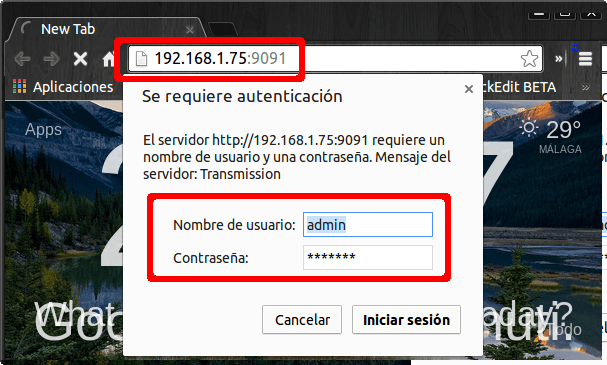
\includegraphics[scale=0.5]{torrent19.png}
\caption{URL y confirmación de acceso}
\label{fig:torrent1}
\end{figure}

\begin{figure}[h!]
\centering
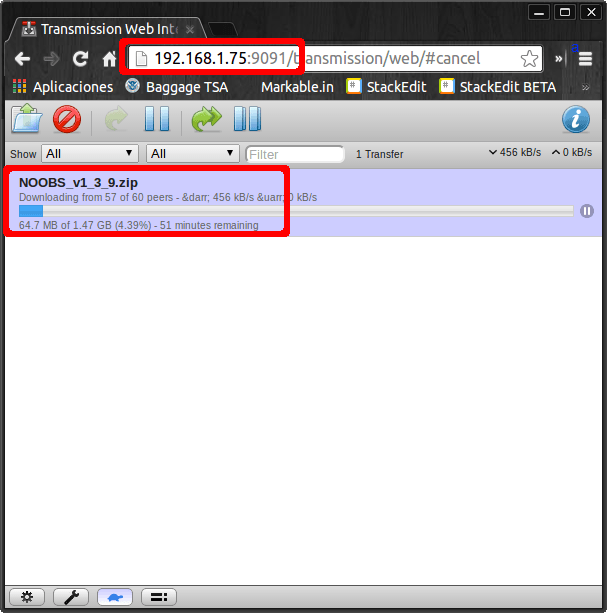
\includegraphics[scale=0.5]{torrent20.png}
\caption{Interfaz de Transmission Web}
\label{fig:torrent1}
\end{figure}



\section{Instalación}
There is a theory which states that if ever anyone discovers exactly what the Universe is for and why it is here, it will instantly disappear and be replaced by something even more bizarre and inexplicable.
There is another theory which states that this has already happened.


\begin{minted}{bash}
  $ wget http://tex.stackexchange.com
  
\end{minted}

\begin{figure}[h!]
\centering

\includegraphics[scale=1.7]{universe.jpg}
\caption{The Universe}
\label{fig:univerise}
\end{figure}

\section{Transmission Server}
Transmission es un programa cliente-servidor para el intercambio de archivos torrents en redes P2P. Para instalarlo, escribiremos este comando:\\

sudo apt-get -y install transmission-daemon
Una vez instalado, arrancará automáticamente, así que para configurarlo adecuadamente, antes hay que detenerlo:\\

\begin{lstlisting}[language=bash]
    $ sudo service transmission-daemon stop
    
\end{lstlisting}

Como lugar donde guardar los torrents, vamos a utilizar un pendrive conectado a la Raspberry Pi (si no lo tenemos instalado, aquí se explica cómo formatearlo y montarlo). Suponiendo que lo tenemos montado en la ruta /media/pen, sólo tendremos que crear dentro de él una carpeta específica para almacenar las descargas y otorgarle luego los permisos adecuados:

\begin{lstlisting}[language=bash] 
    $ cd /media/pen 
    $ sudo mkdir descargas 
    $ sudo chmod 777 descargas

\end{lstlisting}

Hecho lo anterior, ya podemos llevar a cabo la configuración del programa. Para ello editamos el fichero correspondiente:\\

\begin{lstlisting}[language=bash,caption={bash version}]
sudo nano /var/lib/transmission-daemon/info/settings.json
\end{lstlisting}

Las líneas indicadas a continuación son las que debemos editar en este fichero. Al hacerlo, hay que tener en cuenta que, por motivos de seguridad, en rpc-username y rpc-password convendría poner un nombre y una contraseña distintos de los que aparecen por defecto. En cuanto a peer-port y rcp-port estos corresponden, respectivamente, al puerto de conexión para las descargas de torrents	y al puerto de acceso a la interfaz web de Transmission; podemos cambiarlos	o dejar los que vienen por defecto.\\

\begin{lstlisting}[language=bash]
"download-dir": "/media/pen/descargas", 
"incomplete-dir-enabled": false, 
"peer-port": 44027, 
"rpc-authentication-required": true, 
"rpc-bind-address": "0.0.0.0", 
"rpc-enabled": true, 
"rpc-password": "contrasena", 
"rcp-port": 9091, 
"rpc-username": "nombre", 
"rpc-whitelist-enabled": false,
\end{lstlisting}

Guardamos el fichero con los cambios realizados (Ctrl+o, Intro, Ctrl+x), arrancamos de nuevo el servicio:

sudo service transmission-daemon start
y ya podemos acceder mediante el navegador del PC a la interfaz web de descargas de Transmission, escribiendo como dirección la IP local de nuestra Raspberry, seguida por dos puntos (:) y el puerto 9091 indicado antes. Así:

\begin{lstlisting}[language=bash,caption={bash version}]
#!/bin/bash
echo "Hello, world!"
\end{lstlisting}

http://192.168.1.33:9091
En la parte superior veremos una barra de iconos:

\section{Reparar sectores dañados del disco duro con Ubuntu}

Si el disco que queremos reparar es el que contiene el sistema operativo tendremos que hacerlo en modo live porque el disco no puede estar montado, en caso contrario no hace falta. Abrimos una terminal e insertamos el siguiente comando y al final añadiremos la partición que vamos a reparar, por ejemplo si es la partición 3 sería /dev/sda3

sudo fsck -c -y -v /dev/sda

Opciones:

-a. Confirmar automáticamente. No recomendado.
-c. Comprobar bloques en el disco.
-f . Forzar el chequeo aunque todo parezca ok.
-v . (verbose) despliega más información.
-r . Modo interactivo. Espera nuestra respuesta.
-y. Asume yes de respuesta.
También podemos elegir la opción de badblocks arrancando con un live y desde la terminal, añadiendo también al final del comando la partición.

sudo badblocks -s -v -n -f /dev/sda

Opciones:

-s. Nos muestra el proceso de escaneo del disco, mostrándonos los sectores ya chequeados.
-v. Nos indica el modo de escritura utilizado.
-n. Nos pone en modo no destructivo, esto quiere decir que se recuperarán los sectores dañados y la información en el disco duro no será dañada o eliminada.
-f. Reparará los sectores dañados.
Es mejor hacerlo siempre desde modo live ya que puede fallar el sistema y es más seguro. Este proceso puede durar horas pero es bastante efectivo. Una vez terminado el proceso es recomendable formatear para volver a utilizarlo.

Información extraída de Ubuntu y algo más.

\section{Conclusion}
``I always thought something was fundamentally wrong with the universe'' \citep{adams1995hitchhiker}

\bibliographystyle{plain}
\bibliography{references}
\end{document}
